\documentclass[tikz,border=3pt]{standalone}
\usepackage[utf8]{inputenc}
\usepackage[T1]{fontenc}
\usepackage{lmodern}
\renewcommand{\familydefault}{\sfdefault}
\usepackage{sansmath}\sansmath
\usepackage{chemfig}
\usepackage{pgfplots}\pgfplotsset{compat=1.18,/pgf/number format/use comma,/pgf/number format/1000 sep={.}}
\usetikzlibrary{arrows.meta,calc,positioning,decorations.pathmorphing,patterns}
% paleta del sitio
\definecolor{nar}{HTML}{E8680C}\definecolor{narc}{HTML}{FFB35C}\definecolor{hielo}{HTML}{FFF3E8}
\definecolor{tinta}{HTML}{1D1D1F}\definecolor{gris}{HTML}{6E6E73}\definecolor{lila}{HTML}{7C5CF0}
\definecolor{azul}{HTML}{2F6FD6}\definecolor{menta}{HTML}{17A673}\definecolor{coral}{HTML}{E8342A}
\begin{document}
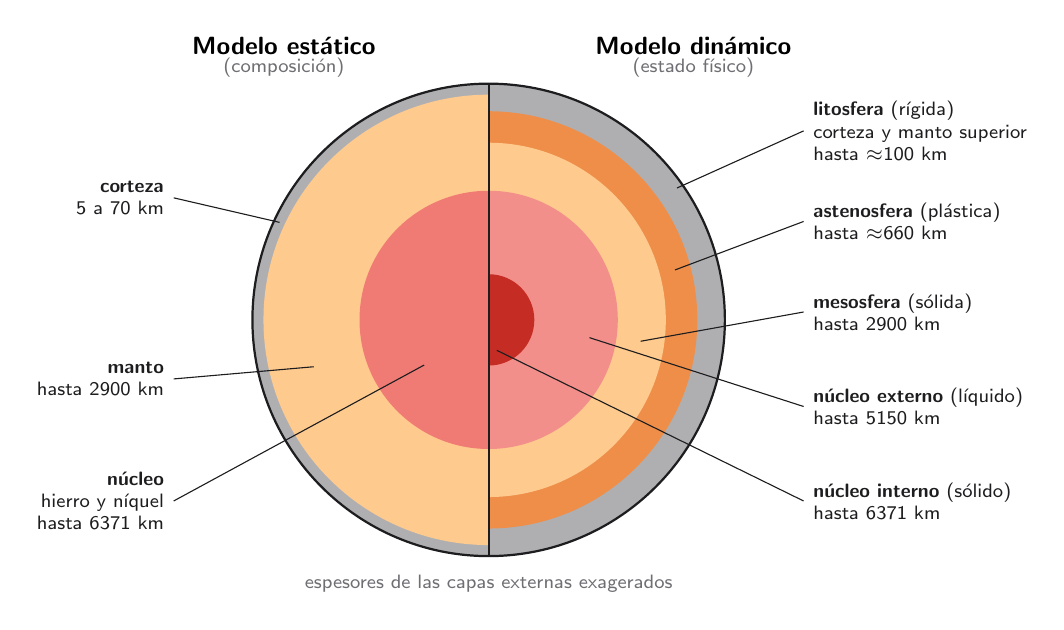
\begin{tikzpicture}[font=\footnotesize]
% radios (capas externas exageradas)
\def\R{3}
% izquierda: modelo estatico
\fill[gris!55] (0,-\R) arc[start angle=-90,end angle=-270,radius=\R] -- cycle;
\fill[narc!70] (0,-2.86) arc[start angle=-90,end angle=-270,radius=2.86] -- cycle;
\fill[coral!65] (0,-1.64) arc[start angle=-90,end angle=-270,radius=1.64] -- cycle;
% derecha: modelo dinamico
\fill[gris!55] (0,-\R) arc[start angle=-90,end angle=90,radius=\R] -- cycle;
\fill[nar!75] (0,-2.65) arc[start angle=-90,end angle=90,radius=2.65] -- cycle;
\fill[narc!70] (0,-2.25) arc[start angle=-90,end angle=90,radius=2.25] -- cycle;
\fill[coral!55] (0,-1.64) arc[start angle=-90,end angle=90,radius=1.64] -- cycle;
\fill[coral!85!black] (0,-0.58) arc[start angle=-90,end angle=90,radius=0.58] -- cycle;
\draw[tinta,thick] (0,0) circle (\R); \draw[tinta,thick] (0,-\R) -- (0,\R);
\node[font=\small\bfseries,anchor=south] at (-2.6,3.25) {Modelo estático};
\node[font=\scriptsize,anchor=south,text=gris] at (-2.6,2.95) {(composición)};
\node[font=\small\bfseries,anchor=south] at (2.6,3.25) {Modelo dinámico};
\node[font=\scriptsize,anchor=south,text=gris] at (2.6,2.95) {(estado físico)};
% etiquetas izquierda
\draw[tinta] (155:2.93) -- (-4.0,1.55) node[left,align=right,font=\scriptsize] {\textbf{corteza}\\5 a 70 km};
\draw[tinta] (195:2.3) -- (-4.0,-0.75) node[left,align=right,font=\scriptsize] {\textbf{manto}\\hasta 2900 km};
\draw[tinta] (215:1.0) -- (-4.0,-2.3) node[left,align=right,font=\scriptsize] {\textbf{núcleo}\\hierro y níquel\\hasta 6371 km};
% etiquetas derecha
\draw[tinta] (35:2.92) -- (4.0,2.4) node[right,align=left,font=\scriptsize] {\textbf{litosfera} (rígida)\\corteza y manto superior\\hasta $\approx$100 km};
\draw[tinta] (15:2.45) -- (4.0,1.25) node[right,align=left,font=\scriptsize] {\textbf{astenosfera} (plástica)\\hasta $\approx$660 km};
\draw[tinta] (-8:1.95) -- (4.0,0.1) node[right,align=left,font=\scriptsize] {\textbf{mesosfera} (sólida)\\hasta 2900 km};
\draw[tinta] (-10:1.3) -- (4.0,-1.1) node[right,align=left,font=\scriptsize] {\textbf{núcleo externo} (líquido)\\hasta 5150 km};
\draw[tinta] (-75:0.4) -- (4.0,-2.3) node[right,align=left,font=\scriptsize] {\textbf{núcleo interno} (sólido)\\hasta 6371 km};
\node[font=\scriptsize,text=gris] at (0,-3.35) {espesores de las capas externas exagerados};
\end{tikzpicture}
\end{document}
